\begin{figure}[t]
  \centering
  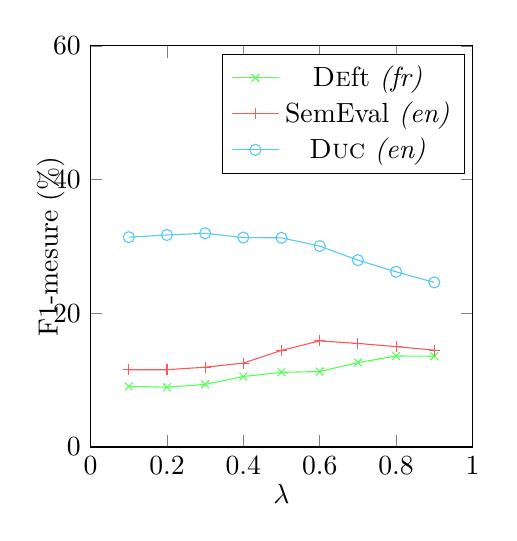
\begin{tikzpicture}
    \pgfkeys{/pgf/number format/.cd, fixed}
    \begin{axis}[x=0.4\linewidth,
                 xtick={0, 0.2, ..., 1.0},
                 xmin=0,
                 xmax=1.0,
                 xlabel=$\lambda$,
                 x label style={yshift=.34em},
                 y=0.007\linewidth,
                 ytick={0, 20, ..., 100},
                 ymin=0,
                 ymax=60,
                 ylabel=F1-mesure (\%),
                 y label style={yshift=-1.1em}]
      \addplot[green!66, mark=x] coordinates{
        (0.1, 9.0736)
        (0.2, 8.9392)
        (0.3, 9.3693)
        (0.4, 10.5436)
        (0.5, 11.1626)
        (0.6, 11.2902)
        (0.7, 12.6269)
        (0.8, 13.6109)
        (0.9, 13.5765)
      };
      \addplot[red!66, mark=+] coordinates{
        (0.1, 11.5509)
        (0.2, 11.5618)
        (0.3, 11.9382)
        (0.4, 12.5558)
        (0.5, 14.4539)
        (0.6, 15.8712)
        (0.7, 15.4920)
        (0.8, 15.0102)
        (0.9, 14.4863)
      };
      \addplot[cyan!66, mark=o] coordinates{
        (0.1, 31.3789)
        (0.2, 31.7112)
        (0.3, 31.9601)
        (0.4, 31.3222)
        (0.5, 31.2842)
        (0.6, 30.0481)
        (0.7, 27.9426)
        (0.8, 26.1973)
        (0.9, 24.6206)
      };
      \legend{\textsc{De}ft \textit{(fr)}, SemEval \textit{(en)}, \textsc{Duc} \textit{(en)}};
    \end{axis}
  \end{tikzpicture}
  \caption{Performance de TopicCoRank, appliqué à \textsc{De}ft, SemEval et
           \textsc{Duc}, lorsque le paramètre $\lambda$ varie
           \label{fig:lambda_variations_general}}
\end{figure}

